% If we assume that a stellar population forms
% impulsively in the distant pass with IMF $\mu(m_*)$(with minimum mass
% $m_0$ and maximum mass $m_1$), then the surviving mass fraction at any
% future time $t$ is given by
% \begin{equation}
% f(t) =\frac{ \int_{m_0}^{m_{\rm T}(t)} m_* \mu(m_*) dm_* }{ \int_{m_0}^{m_1} m_* \mu(m_*) dm_* },
% \end{equation}
% where the main sequence turnoff mass is approximately
% \begin{equation}
% m_{\rm T}(t) \approx 2.5M_\odot~ \left( \frac{t}{10^9~{\rm yr}} \right)^{-0.4}.
% \end{equation}
% For a Salpeter IMF $\mu(m_*) \propto m_*^{-2.35}$ with $m_0=0.1M_\odot$ and $m_1=100M_\odot$,
% \begin{equation}
% f_{\rm Sal}(t) = 1.098 - 0.490 \left(\frac{t}{10^{10}~{\rm yr}} \right)^{0.14}
% \end{equation}
% {\bf NCS: we should probably use a Kroupa/Chabrier IMF, but this gets the ball rolling.}
% If we approximate post-main sequence evolution as instantaneous and define $\lambda(\Mstar)$ as the fractional mass lost during all stages of stellar evolution, then the mass loss rate density
% \begin{equation}
% q(t) = \frac{\rho_*}{\bar{m}_*} \lambda(m_{\rm T}(t)) m_{\rm T}(t) \frac{df}{dt},
% \end{equation}
% where the mean stellar mass $\bar{m}_* = \int_{m_0}^{m_{\rm T}(t)} \Mstar\mu(\Mstar)d\Mstar \approx 0.3 M_\odot$.  Further approximating $\lambda(\Mstar)=0.5$, and using the Salpeter IMF once more, gives
% \begin{equation}
% q(t) = \frac{\rho_*}{10^{10}~{\rm yr}} \times 0.11 \left(\frac{t}{10^{10}~{\rm yr}} \right)^{-1.26}.
% \end{equation}
% This is a specific, time-dependent definition of $\eta(t) (=0.11(t/t_{\rm h})^{-1.26})$; if we consider different star formation scenarios (for example, continuous star formation) or different IMFs, it will change.  Once these free parameters are specified, however, we can answer an important question: do young stellar populations increase or decrease the SMBH feeding rate $\dot{M}$?  Clearly, $\eta(t)$ is larger for young stellar populations, but these stars also have high wind velocities that diminish the stagnation radius.  Crudely approximating $v_{\rm w}=75~{\rm km~s}^{-1}$ for $m_{\rm T} < 10M_{\odot}$ and $v_{\rm w}=3000~{\rm km~s}^{-1}$ for $m_{\rm T} > 10M_{\odot}$ (motivated by the transition from dust-driven wind loss on the AGB to line-driven wind loss from Wolf-Rayet stars), we can employ the relation $\dot{M} \propto \eta(t) r_{\rm s}^{2-\Gamma}\propto \eta(t) v_{\rm w}^{-4+2\Gamma}$ (where $\rho_* \propto r^{-\Gamma}$) to determine the impact of stellar ``youth'' on SMBH feeding rates.
% {\bf AG:As I previously mentioned this discussion of the eta is not
%   quite correct...}
% \begin{figure}
% 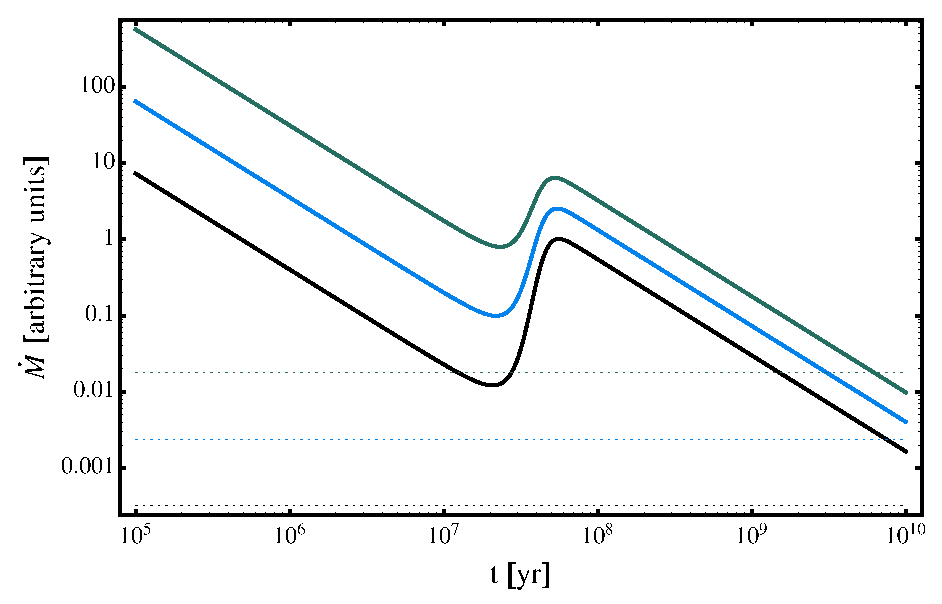
\includegraphics[width=\columnwidth]{NickPlot.eps}
% \caption{\label{NickPlot} SMBH feeding rates $\dot{M}=\eta(t) \times \Mstar(r_{\rm s})$, in arbitrary units.  The green, blue, and black curves are for galaxies with $\Gamma$ values of $0.1$, $0.5$, and $0.9$, respectively.  Solid curves represent impulsive-mode star formation, while dotted curves represent continuous-mode star formation. {\bf NCS: I think these old continuous curves are wrong, need to revise}}
% \end{figure}

% In Fig. \ref{NickPlot} we plot $\dot{M}$, in arbitrary units, as a
% function of time, for three different stellar density profiles $\Gamma
% = \{1.1, 1.5, 1.9\}$ (which are normalized to have the same mass at an
% influence radius $r _{\rm soi}=10~{\rm pc}$ around a $10^7M_\odot$
% SMBH).  We parametrize the wind velocity as
% \begin{equation} \frac{v_{\rm w}}{3000 ~\rm
% km~s^{-1}}=520-495\tanh\left( \frac{t-10^{7.5}~{\rm yr}}{10^{7}~{\rm
% yr}}\right). \label{NickV1}
% \end{equation} This counts Type II SNe heating as ``winds;'' if
% instead we are in the portion of parameter space where $r_{\rm II}$ is
% very large, then we use the alternate parametrization
% \begin{equation} \frac{v_{\rm w}}{3000 ~\rm
% km~s^{-1}}=520-495\tanh\left( \frac{t-10^{7}~{\rm yr}}{10^{6.5}~{\rm
% yr}}\right), \label{NickV2}
% \end{equation} which only allows short lived Wolf-Rayet stars to
% contribute to the high-heating mode.  The ``impulsive burst'' mode of
% star formation produces large ($\sim 10$) differences between the
% three $\dot{M}$ curves at early times, when $r_{\rm s}$ is small, but
% smaller ($\sim 3$) differences at late times, when $r_{\rm s}$ is
% large.  We also plot, as dotted curves, a simple model for the
% ``continuous'' mode of star formation, where mass loss is calculated
% as $\bar{\eta} = \int\eta(t)dt/t_{\rm h} \approx 4$ and an average
% energy injection in the wind is calculated as $\bar{v_{\rm
% w}^2}=\int\eta(t)v_{\rm w}^2(t)dt/\bar{\eta} \approx (800~{\rm
% km~s}^{-1})^2$.  Interestingly, the continuous mode of star formation
% produces small differences from late-time $\dot{M}$ seen in cusp
% galaxies with impulsive star formation; however, continuous mode star
% formation decreases late-time $\dot{M}$ by an order of magnitude
% relative to impulsive star formation in core galaxies.  {\bf NCS: I
% think this old discussion of MDot in the continuous limit is wrong,
% need to revise}

\subsection{Single Burst}

For a stellar population that forms impulsively, the rate of mass and energy injection per unit stellar mass at age $t$ are given, respectively, by 
\begin{align} 
  \dot{\bar{m}}(t) &= \frac{\Delta M(t) \mu|_{M_{\rm TO}(t)}
    \left|\dot{M}_{\rm TO}(t)\right| + f_{\rm MS} \int_{m_0}^{m_{\rm
        T}(t)}
    \dot{m}(\Mstar, t) \mu|_{\Mstar} {\rm d}\Mstar }{\bar{m}_*}\\
  \dot{\bar{e}}(t) &=\dot{e}_{\rm TO}(t)+ f_{\rm MS} \int_{m_0}^{m_{\rm T}(t)}
  \frac{\vw^2(\Mstar, t) \dot{m}(\Mstar, t) \mu|_{\Mstar} {\rm d}\Mstar}{\bar{m}_*},
  \label{eq:edotImp}
\end{align} 
where the first and second terms in each expression corresponds to contributions from main sequence (MS) stars and post-main sequence (PMS) stars, respectively.  Here $ f_{\rm MS} < 1$ is the efficiency with which main sequence winds thermalize their energy with the rest of the injected gas (we hereafter assume $f_{\rm MS} = 1$) and $\mu$ is the IMF, which we take to be of the Salpeter form $\mu(\Mstar)\sim M^{-2.35}$, truncated at $m_0 = 0.1 \Msun$ on the low mass end and at $100 \Msun$ on the high mass end, where $\bar{m}_*$ = 0.35 $\Msun$ is the corresponding mean stellar mass.  

The quantity of mass lost in PMS winds $\Delta M(t)$ is estimated from the expression given by \citet{CiottiOstriker:2007a} (their eq.~[10]),
\begin{align}
\Delta M=
\begin{cases}
0.945 M_{\rm TO}-0.503 & M_{\rm TO} < 9 \Msun\\
 M_{\rm TO}-1.4 \Msun &  M_{\rm TO} \ge 9 \Msun,
\end{cases}
\end{align}
where $M_{\rm TO}$ is the turn-off mass, which at time $t$ is calculated as
\begin{align}
\log(M_{\rm TO})/M_{\odot} =0.24 + 0.068 x^2-0.34 x+4.76 e^{-4.58 x},
\end{align}
where $x=\log(t/10^9 {\rm years})$.  This functional fit is designed to reproduce the results of \citet{MaederMeynet:1987a} (their Table 9) for massive stars while asymptoting to the formula provided by \citet{CiottiOstriker:2007a} (their eq.~[9]) for intermediate and late times ($t \gsim 10^8$ years).

The MS wind mass loss rate $\dot{m}(\Mstar, t)$ is calculated based on the generalization of Reimer's law given in \citet{SchroderCuntz:2005a} (their eq.~[4]) as
\begin{align}
  \dot{m}=8 \times 10^{-14} \frac{L_* R_*}{\Mstar}
  \left(\frac{T_{\rm eff}}{\rm 4000 K}\right)^{3.5}
  \left(1+\frac{g_{\odot}}{4300 g_*}\right) \Msun \pyear,\
\end{align}
where  $R_*$, $L_*$, $T_{\rm eff}$ and $g_*$ are the stellar radius,
luminosity, effective temperature, and surface gravity, respectively, the latter normalized to its solar value $g_{\odot}$.  The stellar radius and luminosity are estimated as (\citet{Kippenhahn&Weigert90}; Figs.~22.2) 22.3)
\begin{align}
L_*=
\begin{cases}
L_{\odot} (\Mstar/\Msun)^{3.2} & \Mstar > \Msun \\
L_{\odot} (\Mstar/\Msun)^{2.5} & \Mstar \le \Msun
\end{cases}
\end{align}
\begin{align}
R_*=
\begin{cases}
R_{\odot} (\Mstar/\Msun)^{0.57} & \Mstar > \Msun \\
R_{\odot} (\Mstar/\Msun)^{0.8} & \Mstar \le \Msun
\end{cases}
\end{align}
The wind velocity of main sequence winds $v_w (\Mstar, t)$ is assumed to equal 430 km s$^{-1}$, corresponding to the escape speed of the Sun; this produces an effective wind heating velocity for main sequence winds alone of $XXX$, in agreement with the value of 150 km s$^{-1}$ found by \citet{NaimanSoares-Furtado+:2013a} based on a more sophisticated population synthesis treatment. {\bf BDM: true? correct}...{\bf AG:Current just use the value for the sun~430 km/s
  replace with the real prescription we end up using.}

The rate of energy input from PMS winds, $\dot{e}_{\rm TO}(t) = f_{8}\dot{\mathcal{E}}/\bar{m}_*$, is dominated by fast Wolf-Rayet winds and core-collapse supernovae from massive stars ($M_{\star} > 8M_{\odot}$), where $f_{8} =2.6 \times 10^{-3}$ is the fraction of the stellar mass with $M_{\star} > 8M_{\odot}$ for our assumed Salpeter IMF.  Here $\dot{\mathcal{E}} (t)$ is the energy injection rate per massive star, which we estimate as
\begin{align}
\dot{\mathcal{E}} (t)=  1.3 \times 10^{36} {\rm erg\,s^{-1}}
\begin{cases}
  1 & t<4 \times 10^6 {\rm yr}\\
  \left(\frac{t}{4 \times  10^6\,{\rm yr}}\right)^{-3.73} & t \ge 4 \times 10^6 {\rm yr},
\end{cases}
\label{eq:voss}
\end{align}
based on the results of \citet{VossDiehl+:2009a} (their Fig.~7, top panel), who use a population synthesis code to simulate the mass and energy injection into the ISM from an OB association.  Although equation~\eqref{eq:voss} is valid only for $t \lsim 10$ Myr, in practice the precise functional form of $\dot{e}_{\rm TO}(t)$ is generally unimportant for our purposes, so we adopt equation~\eqref{eq:voss} as being valid for all times.


The effective wind velocity in the limit of an impulsive star formation may then be written
as 
\begin{align}
\bar{v}_w(t)=2 \dot{\bar{e}}(t)/\dot{\bar{m}}(t)
\label{eq:vwImp}
\end{align}
while {\bf BDM: insert correct expression}
\begin{align}
\eta = \dot{\bar{m}}(t)
\label{eq:vwImp}
\end{align}
We plot $\bar{v}_w(t)$ and $\eta(t)$ in Figures~\ref{fig:vwImp} and XXX.

\begin{figure}
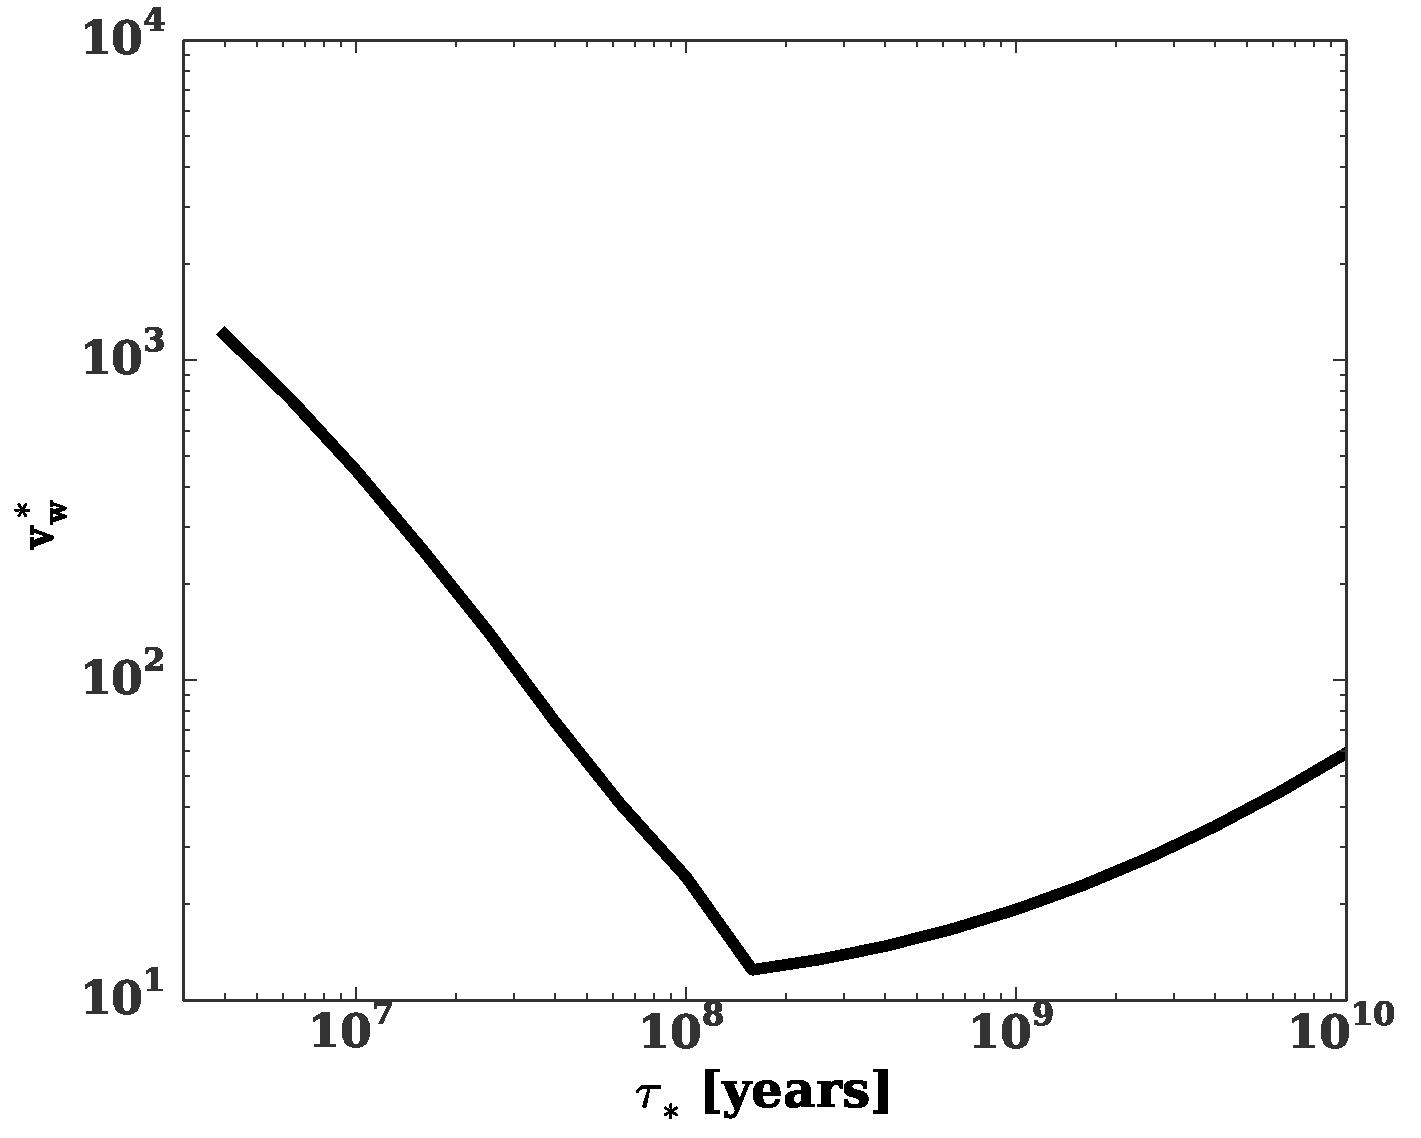
\includegraphics[width=\columnwidth]{vwImp.pdf}
\caption{\label{fig:vwImp} The effective $\vw$ from stellar winds from
  a stellar population of age $t$.}
\end{figure}


\subsection{Over Star Formation History}
Generalizing to an arbitrary star formation history $S(t)$, the total rate of mass and energy input can be written as
\begin{align} 
  \dot{M}(t) &= \int_0^t S(t_1) \dot{\bar{m}}(t-t_1){\rm
      d}t_1\\
  \dot{E}(t) &= \int_0^t S(t_1) \dot{\bar{e}}(t-t_1){\rm
      d}t_1,\\
\end{align}
resulting in an effective wind heating rate of
\begin{align}
  v_w^2(t) &=2 \dot{E}(t)/\dot{M}(t)
\end{align}

\begin{figure}
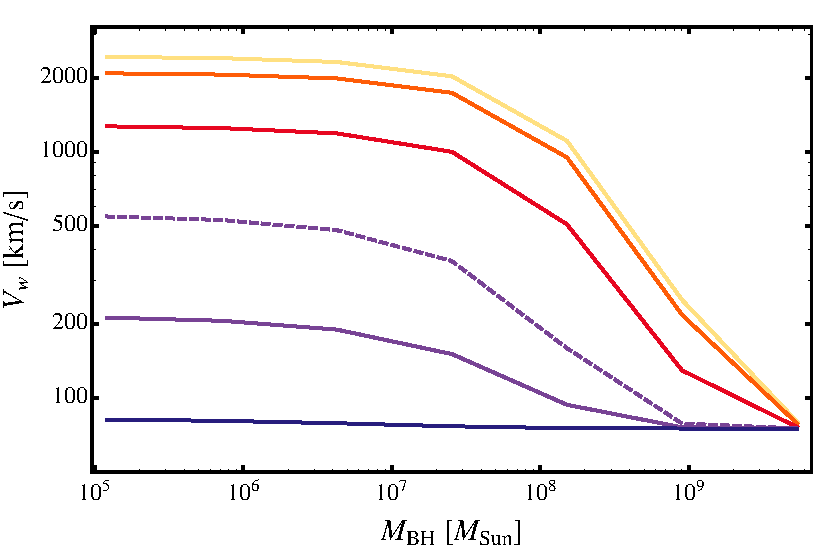
\includegraphics[width=\columnwidth]{vw.pdf}
\caption{\label{NickPlot2} Effective wind velocities $V_{\rm w}$ for
different $S(t)$.  The yellow and orange curves are the Moster SF
histories, with and without Type II SNe, respectively.  The red,
purple, and blue curves are Moster SFs convolved with a $\sin^2(t)$
function normalized to $10^7$, $10^8$, and $10^9$ yr fluctuations,
respectively.  These solid curves lack SN, but the dashed purple curve
possesses it.  Effective $V_{\rm w}$ is strongly diminished when the
variability timescale is greater than $\sim$ twice the duration of
high-velocity winds.}
\end{figure}

We estimate the stellar wind heating provided by the {\it average} star formation history of galaxies of a given mass using the results of \citet{MosterNaab+:2013a} (their eqs.~[17]-[20]) and the $M_{\bullet}-M_{\rm
  halo}$ relation from \citet{BandaraCrampton+:2009a}.  Figure \ref{NickPlot2} shows the resulting $v_{\rm W}$ as a function of SMBH mass.  For comparison we also show cases in which the star formation rate is modulated sinuisoidally from its average value.   It seems that ``bumpy'' SF histories severely diminish $v_{\rm w}$ if the timescale for SF variability is a factor of a few or more greater than the duration of high-velocity winds (either 10 or 40 Myr). {\bf AG: this plot still uses the old ad hoc vw
  prescription? If so it would need to be fixed. In any case, we still
  differ in detail on the vw from stars}.  

%%% Local Variables: 
%%% mode: latex
%%% TeX-master: "ms"
%%% End: 
